\documentclass[12pt, a4paper]{article}

% --- PACKAGES ---
\usepackage[utf8]{inputenc}
\usepackage{geometry}
\usepackage{amsmath}
\usepackage{graphicx}
\usepackage{setspace}
\usepackage{physics}
\usepackage{float}
\usepackage{hyperref}
\usepackage{cite}
\usepackage{tikz}
\usetikzlibrary{shapes.geometric, arrows, positioning}

% --- PAGE SETUP ---
\geometry{left=30mm, top=30mm, bottom=30mm, right=25mm}
\onehalfspacing 

\begin{document}

% ====================================================================
%                             PAGE 1: TITLE PAGE
% ====================================================================
\begin{titlepage}
    \begin{center}
        \vspace*{0.5cm}
        
        % 1. Project Title
        \textbf{\Large \MakeUppercase{Comparative Analysis of Classical
Machine Learning and Quantum
Machine Learning for Predicting
Dengue Outbreaks in Nepal: An
SEIR-Vector Based Approach}}
        
        \vfill
        
        % 2. TU Logo
        \includegraphics[width=4cm]{tulogo.jpg}
        
        \vfill
        
        % 3. Project Type
        \textbf{\large BSC project Proposal}
        
        \vfill
        
        % 4. Submitted To
        Submitted to\\
        Department of Physics \\
        Tri-Chandra Multiple Campus
        
        \vfill
        
        % 5. Submitted By
        By\\
        \vspace{0.3cm}
        \textbf{Roshan Adhikari}\\
        Roll No: 706
        
        \vfill
        
        % 6. Supervisor
        Supervisor\\
        \textbf{Arjun Acharya}\\
        Assist. Professor\\
        Department of Physics\\
        Tri-Chandra Multiple Campus
        
        \vfill
        
        % 7. Date
        \textbf{December 19, 2025}
        \vspace{0.5cm}

    \end{center}
\end{titlepage}
% ====================================================================
%                             PAGES 2-3: Abstract
% ====================================================================
\section*{Abstract}

Dengue fever has rapidly evolved into a major public health challenge in Nepal, driven by urbanization and changing climatic conditions that favor vector increase in higher altitudes. Based on a biophysical understanding of disease transmission, this research proposal describes a comparison between Classical Machine Learning (CML) and Quantum Machine Learning (QML) to forecast dengue outbreaks.

The study uses a hybrid modelling technique based on a compartmental model called Susceptible-Exposed-Infected-Recovered (SEIR-Vector). This model simulates the interactions between human hosts and mosquito vectors using a system of two non-linear ordinary differential equations. The incorporation of daily temperature-dependent parameters for virus incubation and mosquito survival, which represent the thermodynamic limitations of the vector lifecycle, is a significant innovation of this system.

The study employs a multi-scale approach to overcome the biological and computational limitations of forecasting: meteorological and epidemiological data are combined weekly, and the biophysical model is simulated at a daily resolution. The study evaluates the prediction performance of a Quantum Support Vector Machine (QSVM) versus a Classical Random Forest Regressor, with a focus on the time period from 2014 to 2024. The main goal is to determine whether, in comparison to conventional ensemble approaches, the high-dimensional feature spaces made possible by quantum kernels offer a noticeable advantage in capturing the intricate, non-linear lag effects of dengue transmission.

\vspace{0.5cm}
\noindent \textbf{Keywords:} Dengue Fever, SEIR-Vector Model, Random Forest, Quantum Support Vector Machine (QSVM), Epidemiology, Biophysical Modeling.
\newpage
\section*{Acknowledgements}

I want to sincerely thank my supervisor, \textbf{Mr. Arjun Acharya}, for his essential advice, unwavering support, and perceptive criticism during the creation of my thesis proposal. His knowledge has been crucial in determining this project's biophysical and computational course.

Additionally, I would like to express my gratitude to\textbf{ Prof. Pitri Bhakta Adhikari}\,, Head of the Physics Department at \textbf{Trichandra Multiple Campus}, for providing the resources and academic atmosphere needed to carry out this work. My heartfelt gratitude is extended to the entire Department of Physics faculty for their fundamental guidance and assistance.

I would like to acknowledge the \textbf{Epidemiology and Disease Control Division (EDCD)} and \textbf{NASA POWER} for making the epidemiological and meteorological data available, without which this research would not be possible.

Lastly, I want to express my gratitude to my parents and family for their constant patience and support. I also want to thank my friends Sujan Dahal, Sujal Gyawali and Lal Babu Sharma for their encouragement and insightful conversations throughout this process.

\vspace{1cm}
\noindent\textbf{Roshan Adhikari} \\
Roll No: 706 \\
B.Sc. 4th Year Physics \\
Trichandra Multiple Campus

% ====================================================================
%                             PAGES 2-3: CONTENTS
% ====================================================================
\newpage
\tableofcontents
\newpage
\listoffigures
\newpage

% ====================================================================
%                             PAGE 4: INTRODUCTION
% ====================================================================
\section{Introduction}

\subsection{Background}
In Nepal, dengue fever, a virus spread by mosquitoes, has quickly become a significant public health concern. Due to urbanisation and climate change, the virus, which was once limited to the tropical lowlands (Terai), has spread to higher altitudes, including the Kathmandu Valley. The main vectors, Aedes aegypti and Aedes albopictus, are extremely sensitive to thermodynamic factors, especially temperature, which controls the duration of the virus incubation period and their reproduction cycles.

\begin{figure}[H]
    \centering
    \includegraphics[width=0.8\textwidth]{Dengue graph 1.png} % Replace with your image filename
    \caption{Graph Showing the historical trend of dengue virus cases in Nepal (2004 - 2024)}
    \label{fig:my_label}
\end{figure}

% The next paragraph starts here.

Classical Machine Learning (CML) methods, such as Random Forest, have been extensively used in predictive modelling to anticipate disease outbreaks using meteorological data. However, traditional approaches may encounter computational constraints as epidemiological datasets become more complex and multidimensional. Using quantum mechanical concepts such as superposition and entanglement to process data in high-dimensional feature spaces, quantum machine learning (QML), and more especially, algorithms such as the Quantum Support Vector Machine (QSVM) that offers a revolutionary method.

\subsection{Problem Statement}
Nepal's current surveillance systems are primarily reactive, depending on cases reported by hospitals after an outbreak has already started. By neglecting the vector population and the time-lagged impact of temperature on viral incubation, standard mathematical models, like the basic SIR model, frequently oversimplify the dynamics.

Furthermore, it is still uncertain if quantum machine learning can provide a clear benefit in capturing the complex, non-linear interactions inherent in disease transmission, even though classical machine learning has improved predicting accuracy. Comparative studies that thoroughly assess whether the theoretical benefits of quantum computing translate into real-world advancements in Dengue dynamics prediction in the particular setting of Nepal are scarce.


\subsection{Objectives}
Based on a biophysical knowledge of the disease, the main goal of this study is to assess the predictive power of classical and quantum machine learning models for dengue outbreaks. The particular goals are:

\begin{enumerate}
    \item To simulate Dengue transmission dynamics using a \textbf{Biophysical SEIR-Vector Model} that accounts for temperature-dependent incubation periods.
    \item To implement a Classical \textbf{Random Forest Regressor} to predict infection trends using historical weather and case data.
    \item To implement a \textbf{Quantum Support Vector Machine (QSVM)} using a quantum kernel estimator to perform the same prediction task.
    \item To perform a comparative analysis of both models based on prediction accuracy (RMSE), computational cost, and ability to generalize from limited data.
\end{enumerate}

\newpage

% ====================================================================
%                             PAGES 5-6: LITERATURE REVIEW
% ====================================================================
\section{Literature Review}

\subsection{Epidemiological Modeling}
The mathematical foundation of epidemiology was laid by Kermack and McKendrick (1927) with the SIR model \cite{ref1}. However, this model is insufficient for vector-borne diseases. Esteva and Vargas (1998) expanded this to a coupled Vector-Host model, which explicitly accounts for the mosquito population \cite{ref2}. This project builds on their framework by integrating the thermodynamic findings of Watts et al. (1987), who demonstrated that the extrinsic incubation period of the Dengue virus is strictly temperature-dependent \cite{ref3}. This model was termed as the SIER Vector Model.
% Your paragraph text ends here.

\begin{figure}[H]
    \centering
    \includegraphics[width=0.8\textwidth]{seir_vector_diagram.png} % Replace with your image filename
    \caption{SEIR Vector Model Diagram}
    \label{fig:my_label}
\end{figure}

% The next paragraph starts here.

\subsection{Machine Learning in Disease Forecasting}
For epidemic forecasting, Random Forest has become a reliable technique. Benedum et al. (2019) demonstrated that ensemble approaches perform better than basic linear regressions when handling noisy environmental data by successfully using Random Forest to forecast Dengue cases in Peru. \cite{ref4}. Dhimal et al. (2015) found an association between vector distribution and climate factors in Nepal, however these investigations were primarily statistical rather than predictive machine learning. \cite{ref5}.

\subsection{Quantum Machine Learning}
A new field called quantum machine learning (QML) uses quantum processors to analyse data. By introducing the idea of the "Quantum Kernel," Havlíček et al. (2019) showed how quantum computers may effectively compute inner products in Hilbert spaces that are computationally impossible for classical computers. \cite{ref6}. This feature implies that QSVMs may be able to spot minute trends in epidemiological data that traditional kernels could overlook.

\newpage

% ====================================================================
%                             PAGES 7-8: THEORETICAL FRAMEWORK
% ====================================================================
\section{Theoretical Framework}

\subsection{The Biophysical SEIR-Vector Model}
The host (human) and vector (mosquito) populations are modelled in this work using a system of coupled Non-Linear Ordinary Differential Equations (ODEs).
\subsubsection{Human Population Dynamics}
The human population is divided into Susceptible ($S_h$), Exposed ($E_h$), Infected ($I_h$), and Recovered ($R_h$) compartments:
\begin{equation}
    \frac{dS_h}{dt} = - \beta_h S_h I_v
\end{equation}
\begin{equation}
    \frac{dE_h}{dt} = \beta_h S_h I_v - \sigma_h E_h
\end{equation}
\begin{equation}
    \frac{dI_h}{dt} = \sigma_h E_h - \gamma I_h
\end{equation}
\begin{equation}
    \frac{dR_h}{dt} = \gamma I_h
\end{equation}

\subsubsection{Vector Population Dynamics}
The mosquito population includes Susceptible ($S_v$), Exposed ($E_v$), and Infected ($I_v$) compartments, with logistic growth:
\begin{equation}
    \frac{dS_v}{dt} = \Lambda_v - \beta_v S_v I_h - \mu_v S_v
\end{equation}
\begin{equation}
    \frac{dE_v}{dt} = \beta_v S_v I_h - \sigma_v E_v - \mu_v E_v
\end{equation}
\begin{equation}
    \frac{dI_v}{dt} = \sigma_v E_v - \mu_v I_v
\end{equation}

\subsection{Classical ML: Random Forest}
Random Forest is a bagging ensemble method. It aggregates the predictions of $B$ individual decision trees:
\begin{equation}
    \hat{f}(x) = \frac{1}{B} \sum_{b=1}^{B} f_b(x)
\end{equation}
Its capacity to manage non-linear interactions between weather variables (such as temperature and humidity) and its resilience against overfitting are the reasons it was selected.
\subsection{Quantum ML: Quantum Support Vector Machine}
The QSVM maps classical data $\mathbf{x}$ into a quantum state $\ket{\Phi(\mathbf{x})}$ using a feature map. The kernel function is evaluated as the overlap between two quantum states:
\begin{equation}
    K(\mathbf{x}_i, \mathbf{x}_j) = |\braket{\Phi(\mathbf{x}_i)}{\Phi(\mathbf{x}_j)}|^2
\end{equation}
The best separating hyperplane (or regression line) in the high-dimensional feature space is then found using this "Quantum Kernel" in a traditional SVM optimisation procedure.

\newpage

% ====================================================================
%                             PAGE 9: METHODOLOGY
% ====================================================================
\section{Methodology}

\subsection{Tools and Environment}
The research will be conducted on a MacOS-based system using Python.
\begin{itemize}
    \item \textbf{Simulation:} \texttt{SciPy} (solve\_ivp) for integrating the SEIR ODEs.
    \item \textbf{Classical ML:} \texttt{Scikit-Learn} for Random Forest implementation.
    \item \textbf{Quantum ML:} \texttt{PennyLane} for creating quantum circuits and kernel estimation.
\end{itemize}

\subsection{Data Sources}
\begin{enumerate}
    \item \textbf{Epidemiological Data:} Dengue case counts from the Epidemiology and Disease Control Division (EDCD), Nepal. 
    \begin{itemize}
        \item \textbf{Timeframe Selection:} Despite the fact that dengue infections have been documented since 2004, data from 2004 to 2014 shows a low-transmission phase with few, irregular cases. This study will concentrate on the endemic period from 2014 to 2024 in order to guarantee statistical significance and prevent zero-inflation bias in the machine learning models.
        \item \textbf{Temporal Resolution:} Epidemiological case data will be aggregated on a weekly basis, while raw data is available every day. This frequency is selected to maintain a suitable sample size ($\approx 520$ weeks) for Quantum Machine Learning training while matching the biological incubation time of the virus (around 10–14 days).
    \end{itemize}
    
    \item \textbf{Meteorological Data:} Daily temperature ($T_{max}, T_{min}$), rainfall, and humidity obtained from the NASA POWER database.
\end{enumerate}

\subsection{Research Plan}
\begin{itemize}
    \item \textbf{Data Preprocessing:} Cleaning data, handling missing values, and engineering lag features (e.g., Temperature 14 days ago).
    
    \item \textbf{SEIR Calibration:} Tuning the $\beta$ (transmission) and $\sigma$ (incubation) parameters of the mathematical model.
    \begin{itemize}
        \item \textbf{Multi-Scale Simulation Strategy:} The Biophysical SEIR-Vector model will be simulated using a daily time-step ($dt=1$ day) to accurately capture the temperature-dependent mosquito lifecycle. The output of this daily simulation will then be aggregated into weekly totals to match the real-world case data and the input format required for the Machine Learning models.
    \end{itemize}
    
    \item \textbf{Model Training:} 
    \begin{itemize}
        \item Train Random Forest on 80\% of the weekly-aggregated dataset.
        \item Train QSVM using a feature map on the same training set.
    \end{itemize}
    
    \item \textbf{Evaluation:} Compare Root Mean Square Error (RMSE) and R-Squared ($R^{2}$) values on the 20\% test set.
\end{itemize}


\begin{figure}[h]
\centering
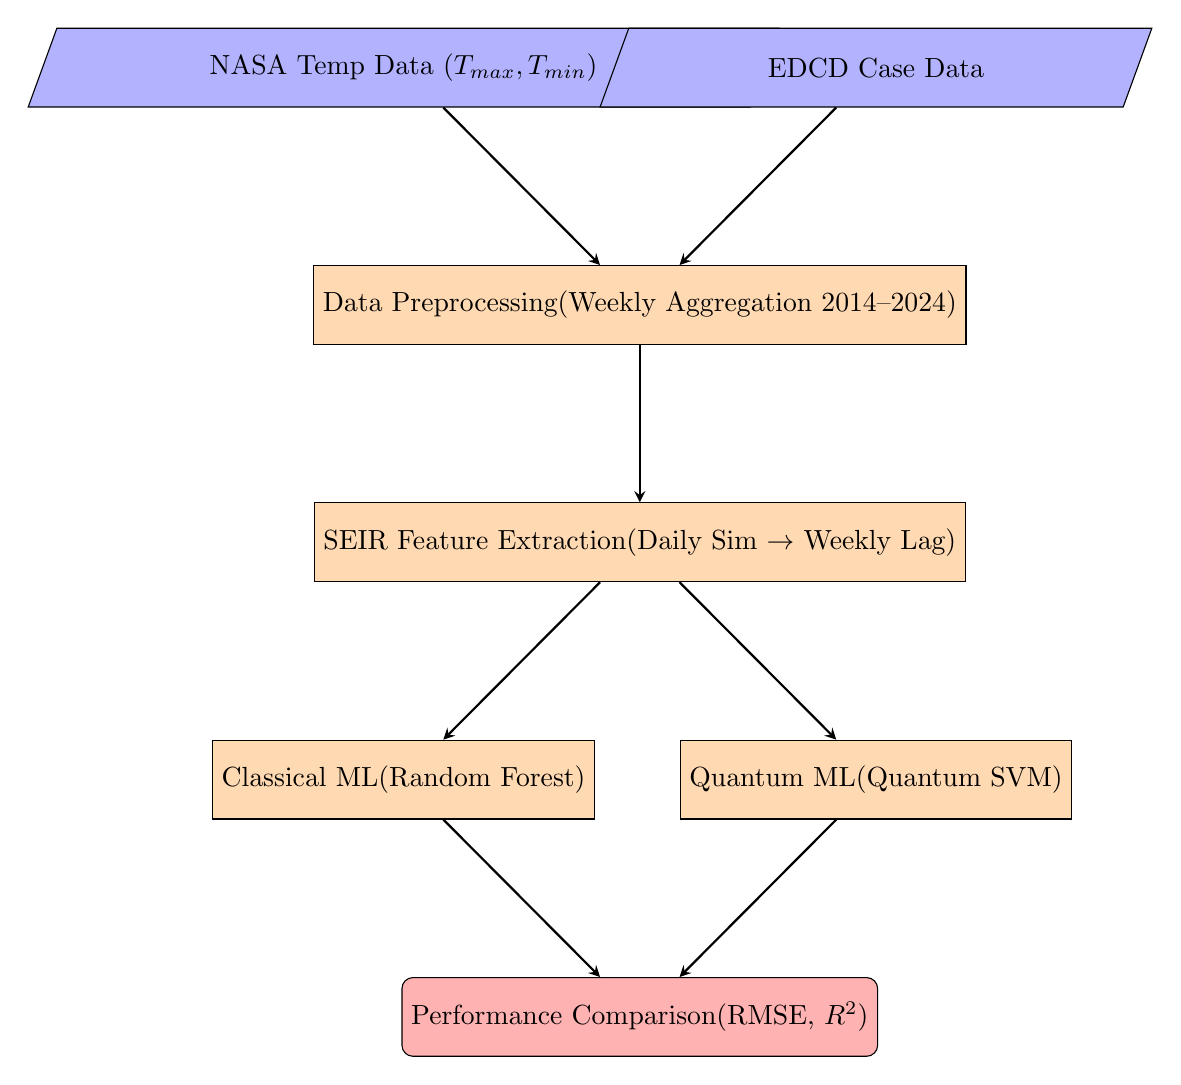
\begin{tikzpicture}[node distance=2cm]

% --- Define Styles ---
\tikzstyle{startstop} = [rectangle, rounded corners, minimum width=3cm, minimum height=1cm,text centered, draw=black, fill=red!30]
\tikzstyle{io} = [trapezium, trapezium left angle=70, trapezium right angle=110, minimum width=3cm, minimum height=1cm, text centered, draw=black, fill=blue!30]
\tikzstyle{process} = [rectangle, minimum width=4cm, minimum height=1cm, text centered, draw=black, fill=orange!30]
\tikzstyle{decision} = [diamond, minimum width=3cm, minimum height=1cm, text centered, draw=black, fill=green!30]
\tikzstyle{arrow} = [thick,->,>=stealth]

% --- Nodes ---
\node (temp) [io] {NASA Temp Data ($T_{max}, T_{min}$)};
\node (case) [io, right of=temp, xshift=4cm] {EDCD Case Data};

\node (process1) [process, below=of temp, xshift=3cm] {Data Preprocessing \\ (Weekly Aggregation 2014--2024)};

\node (seir) [process, below=of process1] {SEIR Feature Extraction \\ (Daily Sim $\rightarrow$ Weekly Lag)};

\node (ml) [process, below=of seir, xshift=-3cm] {Classical ML \\ (Random Forest)};
\node (qml) [process, below=of seir, xshift=3cm] {Quantum ML \\ (Quantum SVM)};

\node (compare) [startstop, below=of ml, xshift=3cm] {Performance Comparison \\ (RMSE, $R^2$)};
% --- Arrows ---
\draw [arrow] (temp) -- (process1);
\draw [arrow] (case) -- (process1);
\draw [arrow] (process1) -- (seir);
\draw [arrow] (seir) -- (ml);
\draw [arrow] (seir) -- (qml);
\draw [arrow] (ml) -- (compare);
\draw [arrow] (qml) -- (compare);

\end{tikzpicture}
\caption{Proposed Research Workflow Methodology}
\label{fig:workflow}
\end{figure}



\newpage

% ====================================================================
%                             PAGE 10: EXPECTED RESULTS
% ====================================================================
\section{Expected Results}

\subsection{Simulation}
It is anticipated that the SEIR-Vector model will show the lag between peak temperature and peak infections, confirming the virus's thermodynamic mechanism.

\subsection{Comparative Analysis}
Because of its maturity, we expect the Random Forest model to offer a high baseline accuracy. In situations with high feature complexity, the Quantum SVM is anticipated to meet or somewhat surpass this accuracy; but, because of simulation cost on classical hardware, it might be computationally slower.

\begin{table}[H]
\centering
\begin{tabular}{|l|c|c|}
\hline
\textbf{Metric} & \textbf{Random Forest} & \textbf{Quantum SVM} \\ \hline
Training Time & Fast & Slower (Simulated) \\ \hline
Accuracy ($R^2$) & High ($>0.85$) & To be evaluated \\ \hline
Data Efficiency & Moderate & Potentially High \\ \hline
\end{tabular}
\caption{Framework for comparing Classical vs Quantum models.}
\end{table}

\newpage

% ====================================================================
%                             PAGE 11: TIMELINE & BUDGET
% ====================================================================
\section{Project Timeline}

\begin{table}[H]
\centering
\renewcommand{\arraystretch}{1.5}
\begin{tabular}{|l|c|c|c|c|}
\hline
\textbf{Task / Month} & \textbf{Month 1} & \textbf{Month 2} & \textbf{Month 3} & \textbf{Month 4} \\ \hline
Literature Review & X & & & \\ \hline
Data Collection & X & & & \\ \hline
SEIR Modeling & & X & & \\ \hline
ML \& QML Coding & & X & X & \\ \hline
Thesis Writing & & & X & X \\ \hline
Final Defense & & & & X \\ \hline
\end{tabular}
\caption{Proposed project schedule.}
\end{table}

\section{Estimated Budget}
\begin{itemize}
    \item \textbf{Internet \& Data:} NRs. 3,000
    \item \textbf{Cloud Resources:} NRs. 2,000
    \item \textbf{Printing \& Binding:} NRs. 4,000
    \item \textbf{Miscellaneous:} NRs. 1,000
    \item \textbf{Total Estimated Cost:} \textbf{NRs. 10,000}
\end{itemize}

\newpage

% ====================================================================
%                             PAGE 12: REFERENCES
% ====================================================================
\begin{thebibliography}{12}

\bibitem{ref1}
Kermack, W. O., \& McKendrick, A. G. (1927). A contribution to the mathematical theory of epidemics. \textit{Proceedings of the Royal Society of London. Series A}, 115(772), 700-721.

\bibitem{ref2}
Esteva, L., \& Vargas, C. (1998). Analysis of a dengue disease transmission model. \textit{Mathematical Biosciences}, 150(2), 131-151.

\bibitem{ref3}
Watts, D. M., Burke, D. S., Harrison, B. A., Whitmire, R. E., \& Nisalak, A. (1987). Effect of temperature on the vector efficiency of Aedes aegypti for dengue 2 virus. \textit{American Journal of Tropical Medicine and Hygiene}, 36(1), 143-152.

\bibitem{ref4}
Benedum, C. M., Shea, K. M., Jenkins, H. E., Kim, L. Y., \& Markuzon, N. (2019). Weekly dengue forecasts in Iquitos, Peru; predictive modeling with meteorological and epidemiological data. \textit{PLOS Neglected Tropical Diseases}, 13(10), e0007790.

\bibitem{ref5}
Dhimal, M., Ahrens, B., \& Kuch, U. (2015). Climate change and spatiotemporal distributions of vector-borne diseases in Nepal. \textit{Parasitology Research}, 114(8), 2817-2828.

\bibitem{ref6}
Havlíček, V., Córcoles, A. D., Temme, K., Harrow, A. W., Kandala, A., Chow, J. M., \& Gambetta, J. M. (2019). Supervised learning with quantum-enhanced feature spaces. \textit{Nature}, 567(7747), 209-212.

\bibitem{ref7}
Adhikari, S. R., \& Supakankunti, S. (2020). Economic burden of Dengue in Nepal. \textit{Journal of Nepal Health Research Council}, 18(3), 475-480.

\end{thebibliography}

\end{document}